In this chapter we introduce and clarify the technical concepts to necessary understand the subsequent chapters. We also introduce the following notation that is used throughout the dissertation:
\begin{itemize}
  \item Given a finite set $\cX$, let $\Delta(\cX)=\{p\in\real^\cX:\sum_x p(x)=1, p(x)\geq 0\;(\forall x)\}$ we denote the probability simplex on $\cX$. 
  \item Given a probability distribution $p\in\Delta(\cX)$, we let $\cB(p)=\{x\in\cX:p(x) > 0\}\subseteq\cX$ denote the support of $p$.
  \item Given a set $\cX$, let$\lvert\cX\rvert$ we denote the cardinality of set $\cX$.
  \item We use capital, non-caligraphic letters to express random variables while their lowercase counterpart represents a realization of such a random variable. E.g: $S_t$ is a random variable that denotes a state at timestep $t$ and $s_0$ is a realization of such random variable.
\end{itemize}
\section{Markov decision processes}
Stochastic sequential decision problems are usually modeled as Markov decision processes (MDPs). Without loss of generality, we restrict our attention to countable MDPs which are formally defined as tuples $\cM=\langle\cS,\cA,\cR,\kernel,\kernel_0\rangle$, where:
\begin{itemize}
  \item $\cS$ is a countable set of states.
  \item $\cA$ is a finite set of primitive actions.
  \item $\cR:\cS\times\cA\times\cS\rightarrow[R_\text{MIN}, R_\text{MAX}]$ is a reward function. Though the reward can also be defined as $\cR:\cS\times\cA\rightarrow[R_\text{MIN}, R_\text{MAX}]$ or $\cR:\cS\rightarrow[R_\text{MIN}, R_\text{MAX}]$, we stick to its most general definition that associates rewards to triplets $(s, a, s')\in\cS\times\cA\times\cS$, and modify it as necessary.
  \item $\kernel:\cS\times\cA\rightarrow\Delta(\cS)$ is a transition function that encodes the probability distribution $\kernel(\cdot\lvert s, a)$ over next states for every $(s, a)\in\cS\times\cA$.
  \item $\kernel_0:\Delta(\cS)$ is the initial state distribution. We assume that $\kernel_0(s)>0\;\forall s\in\cS$.
\end{itemize}

The most general form of the interaction between the learning agent and the environment is depicted in Figure~\ref{fig:rl_loop}. Initially, the environment is in a start state that is sampled from the initial state distribution $S_0\sim\kernel_0$. At any timestep $t$, the agent observes a state $S_t$ and chooses an action $A_t\sim\pi(S_t)$ according to a decision rule $\pi$. Such a decision rule is called policy, and it is a function 
$\pi:\cS\rightarrow\Delta(\cA)$ that maps states to distributions over actions. Once the agent executes action $A_t$ in the environment, it receives a reward $R_{t+1} = \cR(S_t, A_t, S_{t+1})$ and a new state $S_{t+1}\sim\kernel(\cdot\lvert\cS_t, A_t)$. When access to a simulator is available it is a common practice to restart the interaction every some timesteps according to the initial state distribution $\cP_0$. 
\begin{figure}
  \centering
  \includegraphics[width=0.8\textwidth]{figures/background/RL_loop.png}
  \caption{Interaction loop in a Markov decision process. The agent observes current state $S_t$ and chooses $A_t\sim(\cdot\lvert S_t)$. The agent receives a feedback (reward) from the environment and a new state which from the point of view of the agent becomes the new current state. }
  \label{fig:rl_loop}
\end{figure}


The quadruple $(s_t, a_t, r_{t+1}, s_{t+1})$ defines a transition while the sequence of transitions up to a certain timestep, \begin{equation*}
  h_t = (s_0, s_0, r_1, s_1,\dots,r_t,s_t),
\end{equation*}
is called history. We let $\cH$ denote the set of all possible histories. Note that the interaction of an agent with the environment can be described at any time by means of elements $h\in\cH$.

These processes are so-called Markov because the Markov property holds both in the reward and transition probability functions. Formally,
\begin{align*}
  \kernel(s_{t+1}\lvert h_t) &= \kernel(s_{t+1}\lvert s_t, a_t), \\
  \cR(s_t, a_t, s_{t+1}\lvert h_t) &=  \cR(s_t, a_t, s_{t+1}).
\end{align*}
This indicates that at timestep $t$ the reward and next state depends solely on the current state (or state and action), and not the full history. This has an important implication since the current state $s_t$ conveys all the necessary information for the agent to learn how to behave optimally.

There are many ways to design policies, but our previous definition implies that we consider policies that:
\begin{itemize}
  \item are Markovian, in the sense that the choice of the action depends on the current state $s_t\in\cS$ and not the whole trajectory $h_t\in\cH$, 
  \item are stationary, because they remain the same over time. To be more precise, the choice of the action given a state does not depend on the timestep $t$ in which the state is observed,
  \item are stochastic as they represent a distribution over actions. More concretely a distribution $\pi(\cdot\lvert s)$ conditioned on the state $s\in\cS$. 
\end{itemize}
Unless otherwise specified, the policies are assumed to satisfy the characteristics just mentioned. We will also make use of the notion of deterministic policies. These are special cases of stochastic policies in which all the probability mass is put over one single action.

The aim of the learning agent is to come up with policies that optimize some numerical objective. We turn our attention to two optimality criteria: the discounted and the average-reward frameworks. 

In the following sections we describe how we can solve each case when $\kernel$ and $\cR$ are fully disclosed to the agent, via dynamic-programming techniques. This setting, in which the reward and transition functions are known, is also referred to as planning in MDPs.

\subsection{The discounted case}
\label{sec:dp}
In the discounted setting, an optimal policy is such that it maximizes the expected discounted return. The discounted return is given by the sum of discounted rewards, 
\begin{equation}
  G_t = \sum_{i=t} ^\infty \gamma ^ {i-t} \cR(S_i, A_i, S_{i+1}).
  \label{eq:return}
\end{equation}
Here, $0<\gamma<1$ is the discount factor. There are several reasons to use the discount factor, such as giving more credit to rewards closer in time. Notwithstanding, its main purpose is to make the return in Equation~\ref{eq:return} have a finite value.

Given a policy $\pi$, we define its value function, $v^\pi:\cS\rightarrow\real$, as the expected discounted return of being at state $s\in\cS$ and following policy $\pi$
\begin{equation}
  v^\pi(s) = \EEcp{\sum_{i=t} ^\infty \gamma ^ {i-t} R_i}{S_t = s}{\pi}\;\forall s\in\cS, 
\end{equation}
where $R_i$ is a shorthand for $\cR(S_i, A_i, S_{i+1})$. We also define the action-value function, $q^\pi:\cS\times\cA\rightarrow\real$, of a state-action pair as the expected discounted return of being at state $s\in\cS$, choosing action $a\in\cA$ and following policy $\pi$ thereafter,
\begin{equation}
  q^\pi(s, a) = \EEcp{\sum_{i=t} ^\infty \gamma ^ {i-t} R_i}{S_t = s, A_t = a}{\pi}\;\forall (s, a)\in\cS\times\cA.
  \label{eq:def_qfunction}
\end{equation}
We use ${\cR(s, a)} = \kernel(s'\lvert s,a)\cR(s, a, s')$ to denote the mean reward. The value function for state $s\in\cS$ is known to satisfy the following Bellman equations:
\begingroup
\addtolength{\jot}{1em}
\begin{align}
  v^\pi(s) &= \EEcp{\sum_{i=t} ^\infty \gamma ^ {i-t} R_i}{S_t = s}{\pi}, \nonumber \\
           &= \EEcp{\cR(s, A_t, S_{t+1}) + \sum_{i=t+1} ^\infty \gamma ^ {i-t+1} R_i}{S_t = s}{\pi}, \nonumber \\
           &= \sum_a\pi(a\lvert s)\sum_{s'}\kernel(s'\lvert s, a) \Bigg(\cR(a, a, s') +  \EEcp{\sum_{i=t} ^\infty \gamma ^ {i-t+1} R_i }{S_t = s'}{\pi}\Bigg), \nonumber \\
           &= \pi(a\lvert s) \kernel(s'\lvert s, a) \Bigg(\cR(a, a, s') +  \gamma\EEcp{\sum_{i=t} ^\infty \gamma ^ {i-t} R_i }{S_t = s'}{\pi}\Bigg)\nonumber \\
  v^\pi(s) &= \sum_a \pi(a\lvert s)\bigg(\cR(s, a) + \gamma \sum_{s'}\kernel(s'\lvert s, a)v^\pi(s')\bigg).
  \label{eq:vfunction}
\end{align}
And similarly, for the action-value function for state-action pair $(s,a)\in\cS\times\cA$:
\begin{align}
  q^\pi(s, a) &= \EEcp{\sum_{i=t} ^\infty \gamma ^ {i-t} R_i}{S_t = s, A_t = a}{\pi}, \nonumber\\
              &= \EEcp{\cR(s, a, S_{t+1}) + \sum_{i=t+1} ^\infty \gamma ^ {i-t+1} R_i}{S_t = s, A_t = a}{\pi}, \nonumber\\
              &= \kernel(s'\lvert s, a) \Bigg( \cR(s, a, s') + \EEcp{\sum_{i=t+1} ^\infty \gamma ^ {i-t+1} R_i}{S_t = s'}{\pi}\Bigg), \nonumber\\
              &= \cR(s, a) + \gamma \kernel(s'\lvert s, a)  \EEcp{\sum_{i=t} ^\infty \gamma ^ {i-t} R_i}{S_t = s'}{\pi},\nonumber\\
  q^\pi(s, a) &= \cR(s, a) + \gamma \kernel(s'\lvert s, a)v^\pi(s')\;\forall (s, a).
  \label{eq:qfunction}
\end{align}
\endgroup
Combining Equations~\eqref{eq:vfunction} and~\eqref{eq:qfunction} yields
\begin{equation}
  v^\pi(s) = \sum_a \pi(a\lvert s) q^\pi(s, a).
  \label{eq:rel_v_q}
\end{equation}
The goal of the agent is to compute a policy $\pi^*$ that maximizes the expected discounted return. We denote the optimal value and action-value functions attained by an optimal policy as $v^*$ and $q^*$, respectively. Note that the optimal value function and action-value function, considering that the optimal policy is deterministic, are related by
\begin{equation}
  v^*(s) = \max_a q^*(s, a).
  \label{eq:rel_v_q_opt}
\end{equation}
The question is how to obtain such optimal value functions, so we can derive the optimal policy.

First, we describe how we can obtain the value function associated with a policy $\pi$. This procedure is usually known as \textit{policy evaluation}. For such, we declare the following Bellman operator $T^\pi:\real^\cS\rightarrow\real^\cS$ as 
\begin{equation}
  (T^\pi v^\pi)(s) = \sum_a \pi(a\lvert s)\bigg(\cR(s, a) + \gamma\sum_{s'} \kernel(s'\lvert s, a)v^\pi(s')\bigg)\;\forall s\in\cS.
  \label{eq:bo}
\end{equation}
By looking at $v^\pi$ as a vector of the appropriate size, Equation~\ref{eq:bo} can be rewritten in vector form as 
\begin{equation}
  T^\pi v^\pi = v^\pi.
\end{equation}
Therefore, computing the true value of $v^\pi$ requires finding the fixed-point solution of the previous system of linear equations. 

We further introduce the Bellman optimality operator $T^*:\real^\cS\rightarrow \real^\cS$ defined as
\begin{equation}
  (T^* v^*)(s) = \max_a \cR(s, a) + \gamma \sum_{s'} \kernel(s'\lvert s, a)v^*(s')\;\forall s\in\cS,
  \label{eq:boo}
\end{equation}
and this allows us to rewrite~\ref{eq:boo} in vector form:
\begin{equation}
  T ^* v^* = v^*.
  \label{eq:boo_vector}
\end{equation}
The previous expression indicates that the optimal value function $v^*$ is the fixed-point solution of the previous system of equations, which in this case is not linear as it requires a $\max$ operation. 

We  derive the first dynamic-programming algorithm called value iteration~\citep{Bellman1958} from Equation~\ref{eq:boo_vector}. Here, we keep an estimate $v_k$ of the optimal value function which updated iteratively as 
\begin{equation}
  v_{k+1}\gets T^* v_k,
  \label{eq:value_iteration}
\end{equation}
for some arbitrary initialization $v_0$ until $\lvert v_{k+1} - v_k\rvert < \epsilon$, where $\epsilon$ is the user-specified precision. Value iteration can be shown to converge thanks to the contraction mapping theorem. \todo{Add proof in the appendix??}

The idea of the operators can be also applied to the action-value function. Thus, we define the Bellman operator $T^\pi:\real^{\cS\times\cA}\rightarrow\real^{\cS\times\cA}$ and the Bellman optimality operator $T^*:\real^{\cS\times\cA}\rightarrow\real^{\cS\times\cA}$ over action-value functions in the following way:
\begin{equation}
(T^\pi q^\pi)(s, a) = \cR(s, a) + \gamma \sum_{s'} \kernel(s'\lvert s, a)v^\pi(s')\;\forall (s, a)\in\cS\times\cA. 
\end{equation}
\begin{equation}
(T^* q^*)(s, a) = \cR(s, a) + \gamma \sum_{s'} \kernel(s'\lvert s, a)v^*(s')\;\forall (s, a)\in\cS\times\cA.
\end{equation}
Value iteration can also be implemented using action-value function, in that case we keep an estimate $q_k$ and update it iteratively as
\begin{equation}
  q_{k+1}\gets T^* q_k.
\end{equation}
We also introduce the greedy operator $\cG:\real^{\cS}\rightarrow\cA^\cS$ over action-value functions which is defined as 
\begin{equation}
  (\cG)(s) = \argmax_{a\in\cA} q^\pi(s, a) 
\end{equation}
and returns a deterministic, greedy policy with respect to the action-value function which takes the form of 
\begin{equation*}
 \pi(s\lvert s) =
    \begin{cases}
      1 & \text{if $a = \cG q^\pi(s, \cdot)$}\\
      0 & \text{otherwise}.
    \end{cases}       
\end{equation*}
The second dynamic-programming algorithm is \textit{policy iteration}~\citep{Howard1960} which consists of interleaved steps of policy evaluation and policy improvement. This algorithm works as follows:
 \begin{enumerate}[label=(\arabic*)]
  \item Fix some initial policy $\pi_0$.
  \item At each iteration solve $T^{\pi_k} q^{\pi_k} = q^{\pi_k}$ (policy evaluation).
  \item Then derive new policy $\pi_{k+1}\gets\cG q^{\pi_k}$ (policy improvement).
  \item If $\pi_k(s)\neq\pi_{k+1}(s)$ for some $s\in\cS$, repeat (2) and (3).
\end{enumerate}
Policy iteration converges to an optimal policy $\pi^*$.

\begin{example}[The episodic case]
  For certain problems discount factor can be deprecated, and we can set $\gamma=1$ when using a suitable reward function. Consider the extended MDP definition $\cM=\langle\cS,\cA,\cT,\cR,\kernel,\kernel_0\rangle$ where $\cT$ is a set of absorbing, terminal states. This implies that $\kernel(s\lvert s, a) = 1\;\forall a\in\cA$ for any $s\in\cT$. In this type of problems the interaction halts when the agent reaches some $s\in\cT$, and gets restarted to an initial state according to $\kernel_0$. This piece of the interaction is called an episode, therefore the name. This setting usually appears under the names of total-reward, first-exit case or goal-oriented MDP. The return is now expressed as
  \begin{equation*}
    G_t = \sum_{i=0}^T \cR(S_i, A_i, S_{i+1}),
  \end{equation*}
  where $T$ is a random variable that represents the timestep in which agent reaches some terminal state. The value and action-value functions satisfy the Bellman recursions exactly as in Equations~\eqref{eq:vfunction} and~\eqref{eq:qfunction}, respectively. The value function for terminal states is set beforehand. Shortest path problems where there is a goal, terminal state can be modeled with this setting by letting $v^*(g)=0$ where $g\in\cT$ is the goal, terminal state, and $\linebreak\cR(s, a, s')=-1$ for any $(s,a,s')\in\cS\times\cA\times(\cS\cup\cT)$.
\end{example}
\subsection{The average-reward case}
A better way to model continuing tasks is the average-reward setting. Here, the agent seeks a policy that maximizes 
\begin{equation}
  \rho^\pi(s) =\lim_{T\rightarrow\infty}\frac 1 T \mathbb{E}_\pi\left[\sum_{i=t}^T\cR(S_i, A_i, S_{i+1})\right] \;\forall s\in\cS
\end{equation}
which is known as the average-reward per step or gain.

This setting is arguably more complex than the discounted one. Commonly, the following assumptions are made to facilitate the design and analysis of algorithms.
\begin{assumption}
  The MDP $\cM$ is communicating~\citep{Puterman1994}: for each pair of states $s,s'\in\cS$, there exists a stationary policy $\pi$ that has non-zero probability of reaching $s'$ from $s$.
  \label{ass:mdp_communicating}
\end{assumption}

\begin{assumption}
  The MDP $\cM$ is unichain~\citep{Puterman1994}: the transition probability distribution induced by all stationary policies admit a single recurrent class.
  \label{ass:mdp_unichain}
\end{assumption}

If no restrictions are applied over the MDP, it is possible that the agent is unable to visit all states preventing it of learning an optimal policy over those states. On the contrary, with the previous assumptions we can guarantee that the agent explores all states. 

We illustrate the communicating and unichain concepts using the next example. 
\begin{figure}[!h]
  \centering
  \input{figures/background/unichain}
  \caption{A communicating and unichain MDP. $\cS\equiv\{s_0, s_1, s_2, s_3\}$ and there are up to 2 actions available in each state. $P_0(s)$ is $1$ if $s=s_0$ and $0$ otherwise.}
  \label{fig:unichain}
\end{figure}
\begin{figure}[!h]
\centering
\begin{tikzpicture}[node distance=cm,on grid,every initial by arrow/.style={ultra thick,->, >=stealth}]

    \tikzstyle{round}=[thick,draw=black,circle]

    \node[round] (s_0) at (0,0) {$s_0$};
    \node[round] (s_1) at (4,0) {$s_1$};
    \node[round] (s_2) at (2,-2) {$s_2$};
    \node[round] (s_3) at (6,-2) {$s_3$};

    \path[thick,->, >=stealth] (s_0) edge[font=\fontsize{9}{0}][bend left] node [above] {$\kernel(s_1\lvert s_0, a_1)=1$} (s_1);
    \path[thick,->, >=stealth] (s_1) edge[font=\fontsize{9}{0}][bend right] node [left] {$\kernel(s_2\lvert s_1, a_1)=1$} (s_2);
    \path[thick,->, >=stealth] (s_1) edge[font=\fontsize{9}{0}][bend left] node [right] {$\kernel(s_3\lvert s_1, a_2)=1$} (s_3);

    \path[thick,->, >=stealth] (s_2) edge[font=\fontsize{9}{0}][bend right] node [below] {$\kernel(s_3\lvert s_1, a_1)=1$} (s_3);
    \path[thick,->, >=stealth] (s_3) edge[font=\fontsize{9}{0}][bend right] node [above] {$\kernel(s_3\lvert s_1, a_1)=1$} (s_2);
    \path[thick,->, >=stealth, red] (s_2) edge[font=\fontsize{9}{0}] [loop left] node {$\kernel(s_2\lvert s_2, a_2)=1$} (s_2);
    \path[thick,->, >=stealth, red] (s_3) edge[font=\fontsize{9}{0}] [loop right] node {$\kernel(s_3\lvert s_3, a_2)=1$} (s_3);


\end{tikzpicture}
\caption{Modified version of Figure~\ref{fig:unichain} where transition between $s_2$ and $s_0$ is removed and self-loop actions are possible at $s_2$ and $s_3$ (colored in red).}
\label{fig:multichain}
\end{figure}
\begin{example}[Example 1]
Figure~\ref{fig:unichain} shows a communicating and unichain MDP. The MDP is communicating because any stationary policy that assigns non-zero probability to $\pi(a_2\lvert s_2)$ allows the agent to visit any state from any other state in the MDP. A recurrent class is a set of states such that all the states in it communicate exclusively with each other and with no state outside this set. Unichain MDPs are those which for every stationary policy, the policy-induced transition  function, contains a single recurrent class, and a (possibly empty) set of transient states (these are states that the agent stops visiting at some point). Now, think about the policy that assigns $\pi(a_1\lvert s_2)=1$. Such policy contains a single recurrent class that includes states $\{s_2, s_3\}$ (that are visited indefinitely), while $\{s_0, s_1\}$, which are visited just once if we assume that the agent starts at $s_0$, constitute the set of transient states. On the contrary, Figure~\ref{fig:multichain} shows a modified version of the previous in which the resulting MDP is not communicating and not unichain. Clearly, the probability of reaching $s_0$ from $s_2$ is zero. Additionally, the policy that chooses $\pi(a_2\lvert s_2)=1$ and $\pi(a_2\lvert s_3)=1$ creates two recurrent classes; one formed by $s_2$ and the other by $s_3$. In this scenario we say the MDP is multichain.
\end{example}

The aforeintroduced assumptions have some direct consequences that simplify the analysis and algorithms: the value functions are well-defined and that the gain of any policy does not depend on the state, thus, $\rho^\pi(s) = \rho^\pi(s') = \rho^\pi$. We use the latter term to denote the gain of the policy $\pi$.

In the absence of a discount factor, the infinite sum of future rewards might now be unbounded, and so, the value functions. To tackle this, the value and action-value functions are now average-regularized by subtracting the gain. Therefore, the value and action-value functions satisfy the following Bellman equations:
\begin{equation}
  v^\pi(s) = \sum_a \pi(a\lvert s)\bigg(\cR(s, a) - \rho^\pi + \gamma \sum_{s'} \kernel(s'\lvert s, a)v^\pi(s')\bigg)\;\forall s\in\cS. 
\end{equation}
\begin{equation}
  q^\pi(s, a) = \cR(s, a) - \rho^\pi + \gamma \sum_{s'} \kernel(s'\lvert s, a)v^\pi(s')\;\forall (s,a)\in\cS\times\cA. 
\end{equation}
And the following Bellman optimality equations:
\begin{equation}
  v^*(s) = \sum_a \pi(a\lvert s)\bigg(\cR(s, a) - \rho^* + \gamma \sum_{s'} \kernel(s'\lvert s, a)v^\pi(s')\bigg)\;\forall s\in\cS. 
\end{equation}
\begin{equation}
  q^*(s, a) = \cR(s, a) - \rho^* + \gamma \sum_{s'} \kernel(s'\lvert s, a)v^*(s')\;\forall (s,a)\in\cS\times\cA. 
\end{equation}

The Bellman equations and the Bellman optimality equations are related by the expressions given in~\eqref{eq:rel_v_q} and~\eqref{eq:rel_v_q_opt}. The goal of the agent is to find a policy $\pi^*$ for that attains the optimal gain $\rho^*$. 

We redefine the Bellman operators for the value function:
\begin{equation}
  (T^\pi v^\pi)(s) = \sum_a \pi(a\lvert s)\bigg(\cR(s, a) + \sum_{s'}  \kernel(s'\lvert s, a)v^\pi(s')\bigg)\;\forall s\in\cS. 
\end{equation}
\begin{equation}
  (T^* v^*)(s) = \max_a \sum_{s'} \cR(s, a) + \sum_{s'} \kernel(s'\lvert s, a)v^*(s')\;\forall s\in\cS.
\end{equation}

We can use \textit{value iteration} as-is (Equation~\ref{eq:value_iteration}) to compute the optimal value function with the newly defined operators. Unfortunately, the values can grow very large. \textit{Relative value iteration}~\citep{White1963} can be used instead. The idea is to have some reference state $s^*$ whose value is subtracted in every iteration. This modified version of value iteration can be expressed in vector form as
\begin{equation}
    v_{k+1}\gets T^* v_k - T^* v_k(s^*).
\end{equation}
Even though neither of the versions of value iteration computes the optimal gain, this can be computed as 
\begin{equation*}
  \rho^*=v
_{k+1}(s) - v_k(s)
\end{equation*}  when $k\rightarrow\infty$.

Alternatively, the policy iteration scheme previously described can be used to compute the optimal policy in the average-reward case.

\section{Reinforcement learning}
Reinforcement learning (RL) proposes a learning paradigm when the agent is alien to the reward function $\cR$ and the transition probability distribution $\kernel$ of the MDP. In this context, the learning happens through direct interaction with the environment. There is a vast collection of RL algorithms, but besides the intricacies of each method, most of them are built upon the same simple ideas. For the purpose of this dissertation we will limit ourselves to value-based (also known as critic-only in the literature) approaches. These algorithms maintain some estimates of the value function that are updated online using some update rule.

We review the update rules  used by different algorithms in the discounted and average-reward settings in the ensuing sections.

\subsection{The discounted setting}
\citet{Sutton1988} introduces the idea of temporal difference (TD) learning that uses bootstrapping (using predicted values as targets) during learning. The agent interacts with the environment following policy $\pi$ that is kept fixed. The interaction produces samples ${(s_t, a_t, r_{t+1}, s_{t+1})}$ that are used to learn the value function of the given policy in an online manner. The agent maintains an estimate $\widehat v$ of $v^\pi$. The update rule of the so-called TD($0$) algorithm is
\begin{align}
  \delta_t &= r_{t+1} + \gamma \widehat v(s_{t+1}) - \widehat v(s_t)\\  
  \widehat v(s_t) &\gets \widehat v(s_t) + \alpha_t \delta_t,
\end{align}
where the term $\delta_t$ is called the TD error and $\alpha_t$ is the learning rate. This algorithm is said to be on-policy because the policy that is target of the learning is the one used to interact with the environment. 

We can also learn the optimal policy by directly estimating the optimal action-value function using the temporal difference technique. This is the idea of the probably most canonical algorithm in RL, called Q-learning~\citep{Watkins1992}. In this case, the agent keeps an estimate $\widehat q$ of the optimal action-value function $q^*$, and its values are updated using the following scheme:
\begin{align}
  \delta_t &= r_{t+1} + \gamma \max_a \widehat  q(s_{t+1}, a) - \widehat q(s_t, a_t) \\
  \widehat q(s_t, a_t) &\gets \widehat q(s_t, a_t) + \alpha_t \delta_t
  \label{eq:qlearning}
\end{align}
During learning the agent follows an $\epsilon$-greedy policy which with probability $1-\epsilon$ selects the greedy action $(\cG)(s)$, otherwise selects a random exploratory action.
Nonetheless, the target policy is a greedy, deterministic policy over the estimate of the optimal action-value function. Hence, Q-learning is an off-policy method: the policy that is target of the learning and the one used to act in the environment are different.

\subsection{The average-reward setting}

The TD learning scheme can also be applied in the average-reward setting. \citet{Mahadevan1996} gives the average-reward counterpart of the Q-learning algorithm. Now, in addition to maintaining the action-value estimate, we also need to update an estimate $\widehat\rho$ of the optimal gain $\rho^*$. The update rules are as follows
\begin{align}
  \delta_t &= r_{t+1} - \widehat\rho +  \max_a \widehat q(s_{t+1}, a)  - \widehat q(s_t, a_t) \\
  \widehat q(s_t, a_t) &\gets \widehat q(s_t, a_t) + \alpha_t \delta_t \\
  \widehat \rho &\gets \widehat\rho + \beta_t \big(r_t - \widehat\rho + \max_a \widehat q(s_{t+1}, a) - \max_b \widehat q (s_t, b) \big).
  \label{eq:rlearning}
\end{align}
$\alpha_t$ and $\beta_t$ are different learning rates that can be updated independently. The estimate of the gain $\widehat\rho$ is only updated when a non-exploratory action is executed.

\section{Successor features} 
\label{section:successor_features}

Successor features (SF)~\citep{Barreto2017} is a widely used RL representation framework that assumes the reward function is linearly expressible with respect to a feature vector,
\begin{equation}
  \cR^\w(s, a, s') = \w^\intercal\boldsymbol{\phi}(s, a , s').
  \label{eq:reward_sf}
\end{equation}
Here, $\boldsymbol\phi:\cS\times\cA\times\cS\rightarrow\real^{d}$ maps transitions to feature vectors and $\w\in\real^d$ is a weight vector. Every weight vector~$\w$ induces a different reward function and, therefore, a task. 

Following the definition of the action-value function in Equation~\eqref{eq:def_qfunction}, and considering the reward structure introduced in~\eqref{eq:reward_sf}, the action-value function of a state-action pair $(s, a)\in\cS\times\cA$ under policy $\pi$ can be rewritten as
\begin{align}
  q^\pi_\w(s, a) &= \EEcp{\sum_{i=t} ^\infty \gamma^{i-t} \w^\intercal\boldsymbol\phi_i}{S_t = s, A_t = a}{\pi} \nonumber \\
                 & = \w^\intercal\EEcp{\sum_{i=t} ^\infty \gamma^{i-t} \boldsymbol\phi_i}{S_t = s, A_t = a}{\pi} \nonumber \\
                 &=  \w^\intercal \boldpsi^\pi(s, a)
\label{eq:qfunction_sf}
\end{align}
where $\boldsymbol\phi_i = \boldsymbol\phi(S_{i}, A_{i}, S_{i+1})$, and the term
\begin{equation}
  \boldpsi^\pi(s, a) = \EEcp{\sum_{i=t}^\infty \gamma^{i-t} \boldsymbol\phi_i}{S_t = s, A_t = a}{\pi}
  \label{eq:sf}
\end{equation}
constitutes the SF vector of state-action pair $(s,a)\in\cS\times\cA$ under a policy $\pi$, and it represents the expected discounted sum of future feature vectors when following policy $\pi$. The SF vector satisfies a type of Bellman equation 

\begingroup
\addtolength{\jot}{1em}
\begin{align*}
  \boldpsi^\pi(s, a) &= \EEcp{\sum_{i=t} ^\infty \gamma^{i-t} \boldsymbol\phi_i}{S_t = s, A_t = a}{\pi} \\
                     &= \EEcp{\boldsymbol\phi(s, a, S_{t+1}) + \sum_{i=t+1} ^\infty \gamma^{i-t+1} \boldsymbol\phi_i}{S_t = s, A_t = a}{\pi} \\
                     &= \kernel(s'\lvert s, a)\Bigg(\boldsymbol\phi(s, a, s') + \gamma \EEcp{\sum_{i=t} ^\infty \gamma^{i-t} \boldsymbol\phi_i}{S_t = s'}{\pi}\Bigg) \\
                     &= \boldsymbol\phi(s, a) + \gamma \kernel(s'\lvert s, a) \EEcp{\sum_{i=t} ^\infty \gamma^{i-t} \boldsymbol\phi_i}{S_t = s'}{\pi} \\
  \boldpsi^\pi(s, a) &= \boldsymbol\phi(s, a) + \gamma \sum_{a'}\pi(a'\lvert s) \kernel(s'\lvert s, a') \boldsymbol\phi(s', a'),
\end{align*}
\endgroup
where we use $\boldsymbol\phi^\pi(s, a) = \sum_{s'}\kernel(s'\lvert a, s)\boldsymbol{\phi}(s, a, s')$. Therefore, it can be learned with any off-the-shelf RL algorithm such as Q-learning.

SF is a generalization of the successor representation (SR) framework~\citep{Dayan1993} where the feature map $\boldsymbol{\phi}$ is the one-hot encoding of the state space. In this case, SR vector of each state represents a discounted distribution over future next states under policy $\pi$. 

The action value function for a state-action pair $(s, a)$ under policy $\pi$ can be efficiently represented using the SF vector. Due to the linearity of the reward function, the weight vector can be decoupled from the Bellman recursion.
The SF representation leads to \textit{generalized policy evaluation} (GPE) over multiple tasks~\citep{Barreto2020a}, and similarly, to \textit{generalized policy improvement} (GPI) to obtain new better policies~\citep{Barreto2017}.
\subsection{Combining policies in SF}
A family of MDPs is defined as the set of MDPs that share all the components, except the reward function. This set is formally defined as 
\begin{equation*}
    \cM^{\boldsymbol{\phi}}\equiv\{\langle\cS,\cE,\cA,\cR_\w,\mathbb{P}_0, \mathbb{P}\rangle \lvert \cR_\w = \w^\intercal \boldsymbol{\phi}, \forall\w\in\real^d\}.
\end{equation*}

Transfer learning on families of MDPs is possible thanks to GPI. Given a set of policies $\Pi$, learned on the same family~$\cM^{\boldsymbol{\phi}}$, for which their respective SF representations have been computed, and a new task $\w'\in\real^d$, a GPI policy $\pi_{\text{GPI}}$ for any $s\in\cS$ is derived as 
\begin{equation}
    \pi_{\text{GPI}}(s) \in \argmax_{a\in\cA} \max_{\pi\in\Pi} q^\pi_{\w'}(s, a).
    \label{eq:gpi}
\end{equation}

However, there is no guarantee of optimality for $\w'$.
A fundamental question to solve the so-called \textit{optimal policy transfer learning problem}~\citep{Alegre2022} is which policies should be included in the set of policies $\Pi$ so an optimal policy for any weight vector $\w\in\real^d$ can be obtained with GPI. 


\section{Linearly-solvable Markov decision processes}

Linearly-solvable Markov decision processes (LMDPs)~\citep{Todorov2006, Kappen2005} are a restricted class of the more general MDPs where the Bellman optimality equations are linear. This makes the computation of optimal value functions more efficient. In continuous state space domains or contexts of optimal control as probabilistic inference, they frequently appear under the names of path-integral or Kullback-Leibler control~\citep{Kappen2012}. 

Even though this formulation is arguably restricted, the intuition of entropy-regularization \citep{Neu2017}, that lies at the core of LMDPs, is fundamental in RL as it is one of the building blocks of current state-of-the-art deep reinforcement learning algorithms such as trust region policy optimization \citep{Schulman2015}, soft actor-critic (SAC) \citep{Haarnoja2018} or Munchausen RL \citep{Vieillard2020}. In what follows we introduce linearly-solvable Markov decision processes in the finite-horizon (first-exit) setting, its extension to the infinite-horizon (average-reward) setting and we briefly discuss how they can be used along with function approximation.

\subsection{First-exit linearly-solvable Markov decision processes}

We define a first-exit LMDP as a tuple $\cL=\langle\cS,\cT,\kernel,\cR,\cJ\rangle$, where: \begin{itemize}
  \item $\cS$ is a set of non-terminal states.
  \item $\cT$ is a set of terminal states.
  \item $\kernel:\cS\rightarrow\Delta(\cS^+)$ is an uncontrolled transition function, also known as passive dynamics or passive controls.
  \item $\cR:\cS\rightarrow\real$ is a reward function for non-terminal states.
  \item $\cJ:\cT\rightarrow\real$ is a reward function for terminal states.
\end{itemize}

\noindent We let $\cS^+=\cS\cup\cT$ denote the full set of states and $B=\max_{s\in\cS}|\cB(\kernel(\cdot|s))|$ an upper bound on the support of $\kernel$. 

Similarly to the standard RL learning loop, the agent interacts with the environment in a sequential manner. Nonetheless, there are no explicit actions, and now the learning agent follows a policy $\pi:\cS\rightarrow\Delta(\cS^+)$. Such a policy chooses, for each non-terminal state $s\in\cS$, a probability distribution over next states in the support of $\kernel(\cdot|s)$, i.e.~$\pi(\cdot|s)\in\Delta(\cB(\kernel(\cdot|s))$. There is also no explicit mention of the initial state distribution, which is assumed to be uniform over the set of non-terminal states (this is $\kernel_0 = \text{unif}(\cS)$). 

At each timestep $t$, the learning agent observes a state $s_t\in\cS^+$. If $s_t$ is non-terminal, the agent transitions to a new state $s_{t+1}\sim\pi(\cdot|s_t)$ and receives an immediate, regularized reward
\begin{equation*}
  \cR_\eta(s_t, s_{t+1},\pi) = \cR(s_t) - \frac 1 \eta \log \frac {\pi(s_{t+1}|s_t)} {\kernel(s_{t+1}|s_t)},
\end{equation*}
where $\cR(s_t)$ is the reward associated with state $s_t$, and $\eta$ is a temperature parameter. 
%  $\mathrm{KL}(\pi(\cdot|s_t)\Vert\, \kernel(\cdot|s_t))$ is the Kullback-Leibler divergence between $\pi(\cdot|s_t)$ and $\kernel(\cdot|s_t)$ defined as 
% \begin{equation*}
%   \mathrm{KL}(\pi(\cdot|s)\Vert\, \kernel(\cdot|s)) = \sum_{s'} \pi(s'\lvert s) \log \frac{\pi(s'\lvert s)}{\kernel(s'\lvert s)}
% \end{equation*}

Hence the agent can set the probability $\pi(s_{t+1}|s_t)$ freely, but gets penalized by the entropy-regularization term for deviating from the passive controls $\kernel(s_{t+1}|s_t)$, and this penalty is modulated by the temperature parameter $\eta$. On the other hand, if $s_t$ is terminal, the agent receives reward $\cJ(s_t)$ and then the current episode ends. The aim of the agent is to compute a policy $\pi$ that maximizes the expected future \textit{total reward}. For each non-terminal state $s\in\cS$, the value function is defined as
\begin{equation*}
  v^\pi_\eta(s) = \EEc{\sum_{i=t}^{T-1} \cR_\eta(S_i, S_{i+1},\pi) + \cJ(S_T)}{S_t = s, \pi}.
\end{equation*}

Here, $T$ is a random variable representing the time at which the current episode ends, and $S_t$ is a random variable representing the state at time $t$. The expectation is over the stochastic choice of next state $S_{t+1}\sim\pi(\cdot|S_t)$ at each time~$t$, and the time $T$ it takes for the episode to end. It is assumed that the reward of all non-terminal states is negative, i.e.~$\cR(s)<0$ for each $s\in\cS$. As a consequence, $\cR(s,\pi)<0$ holds for any policy $\pi$, and the value $v^\pi_\eta(s)$ has a well-defined upper bound. Note that the value function is computed with respect to a concrete value of the temperature parameter $\eta$.  
%As an alternative to the assumption $\cR(s)<0$, we could instead assume that each policy terminates with probability 1 within a fixed time horizon $H$.


We are interested in finding the optimal policy which implies computing the optimal value function ${v^*_\eta:\cS\rightarrow\real}$, i.e.~the maximum expected future total reward among all policies. The value function is extended to each terminal state $\tau\in\cT$ by defining $v^*_\eta(\tau)\equiv\cJ(\tau)$. The value function $v^*_\eta$ satisfies the Bellman optimality equations:
\begin{align*}
  \eta v^*_\eta(s) &= \eta \max_\pi \left[ \cR(s,\pi) + \mathbb{E}_{s'\sim\pi(\cdot|s)} v^*_\eta(s') \right] \\
  &= \eta \cR(s) + \max_\pi \mathbb{E}_{s'\sim\pi(\cdot|s)} \left[ \eta v^*_\eta(s') - \log \frac {\pi(s'|s)} {\kernel(s'|s)} \right] \;\; \forall s.
\end{align*}
In expectation, the regularization term in reduces to the Kullback-Liebler divergence between $\pi$ and $\kernel$,
\begin{equation*}
  \mathbb{E}_{s'\sim\pi(\cdot|s)} \log \frac {\pi(s'|s)} {\kernel(s'|s)} = \sum_{s'}\kernel(s'\lvert s)\log\frac{\pi(s'\lvert s)}{\kernel(s'\lvert s)} = \mathrm{KL}\big(\pi(\cdot|s)\Vert\, \kernel(\cdot|s)\big).
\end{equation*}

The maximization in the Bellman equations can be resolved analytically~\citep{Todorov2006}, and the optimal value function can be rewritten as
\begin{align*}
  v^*_\eta(s)      &=  \frac 1 \eta \log{\sum_{s'\in\cS}\kernel(s'\lvert s)e^{\eta(\cR(s) + v^*_\eta(s'))})} \;\;\forall s\in\cS, \\
                   &=  \cR(s) + \frac 1 \eta \log{\sum_{s'\in\cS}\kernel(s'\lvert s)e^{\eta v^*_\eta(s')}} \;\;\forall s\in\cS, \\
  \eta v^*_\eta(s) &=  \eta \cR(s) + \log{\sum_{s'\in\cS}\kernel(s'\lvert s)e^{\eta v^*_\eta(s')}} \;\;\forall s\in\cS.
\end{align*}
Now, we introduce the notation $z_\eta(s)=e^{\eta v^*_\eta(s)}$ for each $s\in\cS^+$. We often abuse this notation by referring to $z_\eta(s)$ as the (optimal) value of $s$ and using $z$ instead of $z_\eta$ when the context is clear. After exponentiating, the previous system yields the following Bellman optimality equations that are linear in $z$:
\begin{equation}\label{eq:boe_z_lmdp}
z(s) = e^{\eta\cR(s)} \sum_{s'}\kernel(s'|s)z(s').
\end{equation}
\subsubsection{Solving a first-exit LMDP}
The Bellman equation can be expressed in matrix form by defining a $\lvert\cS\rvert\times\lvert\cS\rvert$ diagonal reward matrix $R=\diag(e^{\eta\cR(\cdot)})$ and a $\lvert\cS\rvert\times \lvert\cS^+\rvert$ stochastic transition matrix $P$ whose entries $(s,s')$ equal $\kernel(s'|s)$. We define a vector $\bf z$ that stores the values $z(s)$ for each non-terminal state $s\in\cS$, and a vector $\bf z^+$ extended to all states in $\cS^+$. The extended vector$\bf z^+$ contains the values of terminal states, which are known due to $\cJ$. Now we can write the Bellman equations in matrix form as:
\begin{equation}\label{eq:eigen_lmdp}
{\bf z} = R P {\bf z^+}.
\end{equation}
Given $z$, the optimal policy $\pi$ is given by the following expression for each pair of states $(s,s')$:
\begin{equation}
\label{eq:lmdp_optimal_policy}
\pi(s'|s) =  \frac {\kernel(s'|s) e^{\eta v(s')} } {\sum_{s''} \kernel(s''|s) e^{\eta v(s'')} } = \frac {\kernel(s'|s)z(s')} {\sum_{s''} \kernel(s''|s)z(s'')}.
\end{equation}

The solution for $z$ corresponds to the largest eigenvector of $RP$.
If the dynamics $\kernel$ and $\cR$ are known, we can apply the power iteration method to Equation~\eqref{eq:eigen_lmdp}~\citep{Todorov2006}.

Alternatively, we can learn an estimate $\widehat{z}$ incrementally using stochastic updates based on state transitions sampled from the uncontrolled dynamics $(s_t,r_t,s_{t+1})$ with the following TD update rule
% use an online algorithm called Z-learning to compute an estimate  \citep{TodorovNIPS2007}. After observing each transition , the update rule of Z-learning is given by
\begin{equation*}
  \widehat{z}(s_t) \gets (1-\alpha_t)\widehat{z}(s_t) + \alpha_t e^{\eta r_t}\widehat{z}(s_{t+1}),
\end{equation*}

where $\alpha_t$ is a learning rate. 
The previous update rule is called \emph{Z-learning}~\citep{Todorov2006} and suffers from slow convergence in very large state spaces and when the optimal policy differs substantially from the uncontrolled dynamics $\kernel$.
%assumes that we sample next states using the uncontrolled transition function $\cP$, which is typically no better than a random walk. 
A better choice is importance sampling, which uses samples from the estimated policy $\widehat{\pi}$ derived from the estimated values $\widehat{z}$ and \eqref{eq:lmdp_optimal_policy} and updates $\widehat{z}$ according to the following update
%to obtain samples that are corrected using the following update~\citet{TodorovPNAS2009}:
%to sample In this case,  suggested a corrected update rule based on importance sampling:
\begin{align}\label{eqn:zlearning-imp}
\widehat{z}(s_t) \gets (1-\alpha_t)& \widehat{z}(s_t) + \alpha_t e^{\eta r_t}\widehat{z}(s_{t+1})\frac {\kernel(s_{t+1}|s_t)} {\widehat{\pi}(s_{t+1}|s_t)}.
\end{align}
However, this requires local knowledge of $\kernel(\cdot|s_t)$ to correct for the different sampling distribution.
%, i.e.~the set of possible next states and their associated uncontrolled probabilities.
Though this seems like a strong assumption, in practice $\kernel$ usually has a simple form, e.g.~uniform distribution.
Further, as shown in \citet{Jonsson2016}, the corrected update rule in \eqref{eqn:zlearning-imp} can also be used to perform off-policy updates in case transitions are sampled using a policy different from $\widehat{\pi}$.
%leading to simultaneous learning of different tasks.
%Note that the expression for the policy $\widehat{\pi}$ in \eqref{eq:pi} and the corrected update rule in \eqref{eqn:zlearning-imp} require local knowledge of $\cP(\cdot|s_t)$, i.e.~the set of possible next states and their associated uncontrolled probabilities. Though this seems like a strong assumption, in practice $\cP$ usually has a simple form, e.g.~uniform. \citet{conf/icaps/Jonsson16} showed that the corrected update rule in \eqref{eqn:zlearning-imp} can also be used to perform off-policy updates in case transitions are sampled using a policy different from $\widehat{\pi}$.

\subsection{Compositionality}
\label{section:compositionality}
\citet{Todorov2009a} introduces the concept of compositionality for LMDPs. Let us consider a set of LMDPs $\{\cL_1,\ldots,\cL_n\}$, where each LMDP $\cL_i=\langle\cS,\cT,\kernel,\cR,\cJ_i\rangle$ has the same components $\cS,\cT,\kernel,\cR$ and only differ in the reward $\cJ_i(\tau)$ of each terminal state $\tau\in\cT$, as well as its exponentiated value $z_i(\tau)=e^{\eta \cJ_i(\tau)}$.

Now consider a new LMDP $\cL=\langle\cS,\cT,\kernel,\cR,\cJ\rangle$ with the same components as the $n$ LMDPs above, except for $\cJ$. Assume that there exist weights $w_1,\ldots,w_n$ such that the exponentiated value of each terminal state $\tau\in\cT$ can be written as
\begin{equation*}
  e^{\eta \cJ(\tau)} = z(\tau) = w_1z_1(\tau) + \ldots + w_nz_n(\tau) = \sum_{i=1}^n w_i z_i(\tau).
\end{equation*}
Since the Bellman optimality equation of each non-terminal state $s\in\cS$ is linear in $z$, the optimal value of $s$ satisfies the same equation:
\begin{equation*}
  z(s) = \sum_{i=1}^n w_i z_i(s).
\end{equation*}
Consequently, if the optimal values $z_1,\ldots,z_n$ of the $n$ LMDPs are previously computed and the weights $w_1,\ldots,w_n$ are known, we immediately obtains the optimal values of the new LMDP $\cL$ without further learning.


\subsection{Average-reward linearly-solvable Markov decision processes}

LMDPs can be extended to the average-reward setting. We say an average-reward Linearly-solvable Markov decision process (ALMDP) is a tuple
$\cL = \langle\cS,\kernel,\cR\rangle$, where $\cS$ is a set of states, $\kernel:\cS\rightarrow\Delta(\cS)$ is the passive dynamics, and $\cR$ is the reward function. ALMDPs represent continuing tasks and, unlike first-exit LMDPs, there are no terminal states. Consequently, there is no reward function for terminal states.  

We restate Assumptions~\ref{ass:mdp_communicating} and~\ref{ass:mdp_unichain} for the case of LMDPs.

\begin{assumption}
  The ALMDP $\cL$ is communicating~\citep{Puterman1994}: for each pair of states $s,s'\in\cS$, there exists a policy $\pi$ that has non-zero probability of reaching $s'$ from $s$.
  \label{ass:communicating}
\end{assumption}

\begin{assumption}
  The ALMDP $\cL$ is unichain~\citep{Puterman1994}: the transition probability distribution induced by all stationary policies admit a single recurrent class.
  \label{ass:unichain}
\end{assumption}
%\todo{I think this assumption is enough: nothe need to introduce the notation for stationary distributions over the state space since we do not use it at any point. This assumption as is is enough to make the gain not to be conditioned by the initial state.}
%{\color{red} \begin{assumption}
%  For all states $s\in\cS$ the reward $\cR(s)$ is bounded in $\left(-\infty, 0\right]$.
%  \label{ass:rewards}
%\end{assumption}}

In the average-reward setting, the value function is defined as the expected average reward when following a policy $\pi:\cS\rightarrow\Delta(\cS)$ starting from a state $s\in\cS$. This is expressed as
\begin{equation}
  v_\eta^\pi(s) = \underset{T\rightarrow\infty}\lim \EEc{\frac{1}{T} \sum_{i=t}^T \cR_\eta(S_i, S_{i+1}, \pi)}{S_t = s, \pi},
  \label{eq:value_function_almdp}
\end{equation}
where $\cR_\eta(s_t, s_{t+1}, \pi)$ is defined as for first-exit LMDPs.
Again, the goal is to obtain the optimal value function $v^*_\eta$. Under Assumption~\ref{ass:unichain}, the Bellman optimality equations can be written as
\begin{equation}
  v^*_\eta(s) = \frac 1 \eta \log{\sum_{s'\in\cS}\kernel(s'\lvert s)e^{\eta(\cR(s) - \rho + v^*_\eta(s'))}} \;\;\forall s\in\cS,
  \label{eq:boe_almdp}
\end{equation}
where $\rho$ is the optimal one-step average reward (i.e.~gain), which is state-independent for unichain ALMDPs~\citep{Todorov2006}. Exponentiating yields
\begin{equation}
  z(s) = e^{\eta(\cR(s) - \rho)} \sum_{s'\in\cS}\kernel(s'\lvert s)z(s') \;\;\forall s\in\cS.
  \label{eq:boe_z_almdp}
\end{equation}
For the optimal value function $z$, the optimal policy is given by the same expression as in~\eqref{eq:lmdp_optimal_policy}.

\subsubsection{Solving an ALMDP}

We let $\Gamma=e^{\eta\rho}$ denote the exponentiated gain. Similar to the first-exit case, we can express Equation~\eqref{eq:boe_z_almdp} in matrix form as
\begin{equation}\label{eq:rel_opt}
  \Gamma {\bf z} = R P {\bf z},
\end{equation}
where the matrices $P\in \real^{\lvert\cS\rvert\times\lvert\cS\rvert}$ and $R\in \real^{\lvert\cS\rvert\times\lvert\cS\rvert}$ are appropriately defined as in~\eqref{eq:eigen_lmdp}. The exponentiated gain $\Gamma$ can be shown to correspond to the largest eigenvalue of $RP$~\citep{Todorov2009}.
An ALMDP can be solved using {\em relative value iteration} by selecting a reference state $s^*\in\cS$, initializing $\widehat{\bf z}_0={\bf 1}$ and iteratively applying
\begin{equation*}
  \widehat{\bf z}_{k+\frac 1 2} \gets R P \widehat{\bf z}_k, \quad \quad \widehat{\bf z}_{k+1} \gets \widehat{\bf z}_{k+\frac 1 2} / \widehat z_{k+\frac 1 2}(s^*).
\end{equation*}
The reference state $s^*$ satisfies $z(s^*)=1$, which makes the optimal value $z$ unique (else any constant shift preserves optimality). After convergence, the exponentiated gain equals $\Gamma=\widehat z_{k+\frac 1 2}(s^*)$. Under Assumption~\ref{ass:communicating}, relative value iteration converges to the unique optimal value $z$~\citep{Todorov2009}.

Analogously to first-exit LMDPs, when $\kernel$ and $\cR$ are not known, the agent can learn estimates $\widehat z$ and $\widehat\Gamma$ of the optimal value function and the exponentiated gain in an online manner, using samples $(s_t, r_t, s_{t+1})$ generated when following the estimated policy $\widehat\pi$. The update rules for the so-called \textit{differential Z-learning} algorithm are given by \todo{Move it to the chapter?}
\begin{align}
  \widehat{z}(s_t)  \gets \widehat{z}(s_{t}) & + \alpha_t \Bigg(\frac{e^{\eta r_t}}{\widehat\Gamma_t}\dfrac{\kernel(s_{t+1}\lvert s_t)}{\widehat\pi_t(s_{t+1}\lvert s_t)}  - \widehat z(s_t)\Bigg),\label{eq:diff_update_z}  \\   %\delta^z_t \\
  \widehat\Gamma_{t+1}    \gets \widehat\Gamma_t       & + \beta_t \Bigg(\frac{e^{\eta r_t}}{\widehat z_t(s_t)}\dfrac{\kernel(s_{t+1}\lvert s_t)}{\widehat\pi_t(s_{t+1}\lvert s_t)}  - \widehat \Gamma_t\Bigg).\label{eq:diff_update_gamma}
\end{align}
The learning rates $\alpha_t$ and $\beta_t$ can be chosen independently.

Unlike the first-exit case, the compositionality property does not hold in the average-reward case.

\subsection{Function approximation in LMDPs}

So far, we have introduced methods for solving (A)LMDPs in the tabular case, where the full state space can be enumerated and stored in memory. However, in cases where the state space is considerably large, tabular methods are unfeasible, and the value function is approximated.

In this line,~\citet{Todorov2010} prescribes two families of methods for adapting LMDPs in the average-reward setting to function approximation. The first one lies in the family of policy gradients while the second ones can be considered critic-only approaches. Here a valid parameterization of the policy $\pi(s'\lvert s, \w)$ is considered.

The Bellman equation~\eqref{eq:boe_almdp} can be rewritten as follows:
\begin{equation}
\label{eq:boe_for_pg}
\rho + v^*(s) =\cR(s) +\log{\sum_{s'\in\cS}\kernel(s'\lvert s)e^{v^*(s')}} \;\;\forall s\in\cS,
\end{equation}
where for the sake of simplicity we assume that $\eta=1$. 

The first flavor of methods builds on the policy gradient theorem for ALMDPs~\citep[cf.~Theorem 1]{Todorov2010} that states that the gradient of the gain in ALMDPs is
\begin{equation}
  \nabla_\w \rho = \sum_{s}\mu(s, \w) \sum_{s'} \nabla_\w \pi(s'\lvert s, \w)\Big( \log \frac{\pi(s'\lvert s, \w)}{\kernel(s'\lvert s)} + \widetilde v(s', \mathbf{r})\Big),
\end{equation}
where $\mu(x, \w)$ is the stationary distribution induced by $\pi$, and $\widetilde v(s,\mathbf{r})$ is an approximation to the (optimal) value function with parameterization $\mathbf r$.

For the second type of methods one could use \textit{approximate} value iteration or \textit{approximate} policy iteration to iteratively improve the weight vector $\w$, even though this results in a biased estimator. An even more direct approach is to use Gauss-Newton method to fit the weight vector $\w$ by directly optimizing~\eqref{eq:boe_for_pg}.

Despite the correctness of the theoretical results, which guarantee that function approximation can be used along with LMDPs, they are of little practical use. Even in the linear function approximation (LFA) case, the policy gradient approach is intricate and unusual. \guillermo{To find the parameterization $\widetilde v(s,\mathbf{r})$, a previous step of finding a projection $\widetilde v(s,\mathbf{s})$ of $v^*$ using a different set of policy-dependent features is required. The process is not as direct as in traditional MDPs and, additionally, the representation of the policy still depends on the size of the whole state space. This makes the approach intractable for real-world problems as it does not scale with large state spaces.}


\section{Hierarchical reinforcement learning}
Hierarchical reinforcement learning (HRL) embodies the idea of divide-and-conquer paradigm in sequential decision problems. This algorithmic paradigm hypothesizes that breaking down a problem into smaller (sub)problems should facilitate its solution, by solving the small problems in isolation and then combining them to give an overall solution. But the philosophical motivations go beyond this as human thinking process happens at different timescales while at the same time we can use the same piece of knowledge to solve different, but similar tasks. Think, for example, about cooking a recipe. This human activity involves different steps than can be solved in isolation such as shopping the ingredients, cutting and chopping vegetables, using the stove or placing the final outcome in plates. A specific sequence of these steps with certain ingredients leads to a unique result, though many of these steps can transfer from recipe to recipe.

We review how the modelling of these (sub)problems are commonly addressed in the context of RL and the issues that they usually entail regarding the optimality of the final solution.

\subsection{The options framework}

\begin{figure}
  \centering
  \includegraphics{figures/background/RL loop with Option.png}
  \caption{The interaction loop in a semi MDP where the underlying MDP is extended with options.}
  \label{fig:options}
\end{figure}

\label{section:options}
A common way to model (sub)problems\footnote{I use the nomenclature (sub)problem with the prefix sub in parentheses to highlight that, even though these problems are part of a bigger one, they are well-defined problems that can be solved in isolation.} in RL is by using the options framework. A Markovian option represents a temporally-extended action and is a tuple $\omega=\langle\cI, \mu, f\rangle$ where:
\begin{itemize}
  \item $\cI\subseteq\cS$ is the initiation set, i.e.~all the states in which the option $\omega$ can be called.
  \item $\mu:\cS\rightarrow\cA$ is the option's policy.
  \item $f:\cS\rightarrow\Delta(\{0, 1\})$ is a termination function.
\end{itemize}
The combination of an MDP $\cS$ with a fixed set of options $\Omega$ results in a semi-MDP $\widetilde\cM=\langle\cS,\Omega, \cR, \kernel, \kernel_0\rangle$, and now, unlike the regular MDP formulation, the agent learns a policy over the space of options $\pi:\cS\rightarrow\Delta(\Omega)$. The interaction is now slightly modified (see Figure~\ref{fig:options}). At timestep $s_t$, the agent selects an option according to policy $\pi$ conditioned on that option being available at that state(i.e.~$s_t\in\cI_\omega$). Such an option that takes control for period of time and that is run until termination. After $T$ timesteps, where $T$ is a random variable representing duration of the option, the control is returned to the agent which then can choose a new option. Note that primitive actions can be considered a special case of options that terminate after one timestep.

We have only described Markovian options. There are cases in which we might want to include a timeout so that the options terminate surely after a certain number of steps. In that case, the options' policies should not only consider the current state, but the history since the option was initialized. We do not go in detail as they these type of options are out of the scope of this dissertation.


In order to write the Bellman equations for the semi MDP formulation, we need to make use of the reward and transition multi-time model~\citep{Sutton1999} induced by the option. These are defined as
\begin{align}
  \cR(s, \omega) &= \mathbb{E}_\mu\bigg[\sum_{i=t}^{t+T}R_i\lvert S_t=s\bigg],\\
  \kernel(s'\lvert s, \omega) &= \sum_{k=0} \gamma^k \text{Pr}(s_k = s'\lvert s,\omega),
\end{align}
where $\text{Pr}(s_k = s'\lvert s,\omega)$ represents the probability that option $\omega$ terminates in state $s'\in\cS$ in exactly $k$ timesteps according to the underlying MDP transition function. Using this extended model, we can write the counterparts of Bellman equations for the value function
\begin{equation}
  v^\pi(s) = \sum_{\omega\in\Omega}\pi(\omega\lvert s)\bigg(\cR(s,\omega) + \sum_{s'}\kernel(s'\lvert s, \omega)v^\pi(s')\bigg),\\
\end{equation}
and the Bellman equations for the action-value function
\begin{equation}
  q^\pi(s, \omega) = \cR(s,\omega) + \sum_{s'}\kernel(s'\lvert s, \omega)v^\pi(s').\\
\end{equation}
By defining the proper Bellman operators, with little modification we can use the dynamic-programming algorithms discussed in section~\ref{sec:dp}.

Similarly, we can learn the optimal policy by letting the agent interact directly with the environment. In this case, the update rule for the Q-learning counterpart with options is
\begin{align}
  \delta_t &= r^o_t + \gamma^k \max_{\omega} q(s_{t+k}, \omega) - q(s_t, \omega_t),\\
  \widehat q(s_t, \omega_t) &\gets \widehat q(s_t, \omega_t) + \alpha_t \delta_t.
\end{align}
Here, $r^o_t = \sum_{i=t}^{t+k}\gamma^{i-t}R_i$ is the cumulative discounted reward achieved by the option, and $k$ is the number of timesteps the option takes to terminate.

\subsubsection{Intra-task learning}
Up to this point, the options have been assumed to be learned before computing the optimal value functions. We can also learn the options' models on the fly while interacting online with the environment. In addition, any sample $(s_t, a_t, r_{t+1}, s_{t+1})$ obtained by executing one option can be used to update the policies of other options consistent with that transition.

\subsection{Optimality of HRL algorithms}
 
\begin{figure}
  \centering
  \input{figures/background/recursive_optimality}
  \hspace{25pt}
      \begin{adjustbox}{width=0.35\textwidth}
    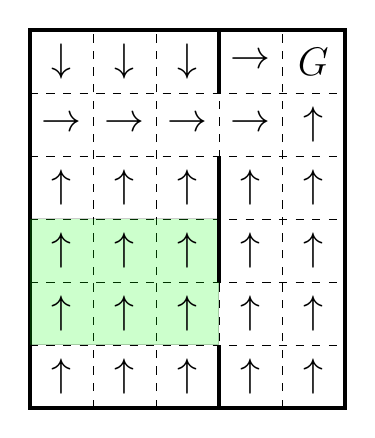
\begin{tikzpicture}
    \draw[step=0.8,ultra thin, dashed] (0,0) grid (4,4.8);
    \draw[ultra thick] (0,0) rectangle (4,4.8);

    \draw[fill=green,opacity=0.2] (0,0.8) rectangle (2.4,2.4);


    \draw[ultra thick] (2.4,0) -- (2.4,0.8);
    \draw[ultra thick] (2.4,1.6) -- (2.4,3.2);
    \draw[ultra thick] (2.4,4) -- (2.4,4.8);

    \node at (3.6,4.4) {\Large $G$};
    \node at (0.4,0.4) {\Large $\uparrow$};
    \node at (1.2,0.4) {\Large $\uparrow$};
    \node at (2,0.4) {\Large $\uparrow$};
    \node at (2.8,0.4) {\Large $\uparrow$};
    \node at (3.6,0.4) {\Large $\uparrow$};
    
    \node at (0.4,1.2) {\Large $\uparrow$};
    \node at (1.2,1.2) {\Large $\uparrow$};
    \node at (2,1.2) {\Large $\uparrow$};
    \node at (2.8,1.2) {\Large $\uparrow$};
    \node at (3.6,1.2) {\Large $\uparrow$};

    \node at (0.4,2) {\Large $\uparrow$};
    \node at (1.2,2) {\Large $\uparrow$};
    \node at (2,2) {\Large $\uparrow$};
    \node at (2.8,2) {\Large $\uparrow$};
    \node at (3.6,2) {\Large $\uparrow$};

    \node at (0.4,2.8) {\Large $\uparrow$};
    \node at (1.2,2.8) {\Large $\uparrow$};
    \node at (2,2.8) {\Large $\uparrow$};
    \node at (2.8,2.8) {\Large $\uparrow$};
    \node at (3.6,2.8) {\Large $\uparrow$};

    \node at (0.4,3.6) {\Large $\rightarrow$};
    \node at (1.2,3.6) {\Large $\rightarrow$};
    \node at (2,3.6) {\Large $\rightarrow$};
    \node at (2.8,3.6) {\Large $\rightarrow$};
    \node at (3.6,3.6) {\Large $\uparrow$};

    \node at (0.4,4.4) {\Large $\downarrow$};
    \node at (1.2,4.4) {\Large $\downarrow$};
    \node at (2,4.4) {\Large $\downarrow$};
    \node at (2.8,4.4) {\Large $\rightarrow$};
    
    \end{tikzpicture}
    \end{adjustbox}
  \caption{Example of a recursively optimal policy (left) and a hierarchically optimal one (right) in a . The area in green highlights the states in which policies disagree.}
  \label{fig:hrl_optimality}
\end{figure}


Most hierarchical algorithms~\citep{Dietterich2000,Parr1997} are known to suffer from suboptimality when providing an overall solution by combining the solution for the (sub)problems. \citet{Dietterich2000} distinguishes two types of optimality for hierarchical methods in reinforcement learning, namely \textit{recursive optimality} and \textit{hierarchical optimality}. Recursive optimality refers to hierarchical algorithms that attain locally optimal solution for each subtask according to the high-level. Though the solution to each independent (sub)problem is indeed optimal, the overall solution is not. Hierarchical optimality, on the other hand, is a stronger concept that implies optimality with regard a constrained space of policies, given by the hierarchy structure.

\begin{example}[Example 2] We recover the example in~\citep{Dietterich2000}. Figure the gridworld environment depicted in Figure~\ref{fig:hrl_optimality}. There are two rooms (left and right) separated by a wall with two doors. The primitive actions $\cA\equiv\{\text{\texttt{left,up,right,down}}\}$, though the agent has only access to two options. The first is \texttt{EXIT ROOM} when the agent is placed somewhere in the left room. The agent can execute a second option \texttt{GO TO G} when it finds itself in the room on the right.  
\end{example}


\section{Non-Markovian task specification}
\label{section:non_markovian}
 {\color{blue}
 
 \begin{itemize}
 \item Difficulty about expressing some tasks in Markovian terms 
 \item Finite State automata and Reward Machines 
 \item Reward Machines and their relationship with logics
 \item Comment on algorithms given in the 
  
\end{itemize}
 
 }


